%% tp3.tex — Presentacion SdS TP3: dinamica molecular regida por eventos (billar-metegol)
%%
%% Compilar desde presentaciones/tp3/:  pdflatex tp3.tex   (dos veces)
%% Estilo: ../sdsbeamer.sty (por \input@path, sin symlink).
%% Figuras: ../../tp3-event-driven-md/analysis/figures/  y  figuras/ (locales: fotogramas)
%% Animaciones: fotograma + link (el PDF de entrega no lleva video embebido).
%%
%% Duracion: 13 min. Estado: 1.1, 1.2 y 1.3 (DCM / D) armados.
%% 1.2 (devolucion de la catedra): tres familias, cada una con animacion -> F_g(t) -> <t_90> vs
%%   variable: disco central -> bloque central -> bloque con filas; cierra con la mejor de cada
%%   familia y la configuracion elegida. Los esquemas de cada familia van en Simulaciones.

\documentclass[aspectratio=169]{beamer}
\makeatletter\def\input@path{{../}}\makeatother
\usepackage{sdsbeamer}
\usepackage{tikz}
\usetikzlibrary{arrows.meta,positioning,calc}
\microtypesetup{expansion=false}

\graphicspath{{../../tp3-event-driven-md/analysis/figures/}{figuras/}}

% Fotograma fijo representativo + enlace explicito debajo (GuiaPresentaciones 2.4.8).
\newcommand{\yt}[1]{\href{https://youtu.be/#1}{\texttt{youtu.be/#1}}}
\newcommand{\animbox}[3]{%
  \centering
  \includegraphics[width=0.9\linewidth]{#1}\par\vspace{0.3em}
  {\small #2}\par\vspace{0.15em}
  {\scriptsize #3}\par
}
\newcommand{\figura}[1]{%
  \centering
  \includegraphics[width=\linewidth,height=0.78\textheight,keepaspectratio]{#1}%
}
% Una sola animacion: fotograma grande + valor de la variable + enlace.
\newcommand{\animsola}[3]{%
  \centering
  \includegraphics[width=0.62\linewidth]{#1}\par\vspace{0.3em}
  {\small #2}\par\vspace{0.15em}
  {\large #3}\par
}

\title{Billar-metegol: dinámica molecular regida por eventos}
\subtitle{Simulación de Sistemas - ITBA}
\author[Grupo 2]{%
  Arancibia Nicolás -- Legajo 64481\\
  Morantes Agustín -- Legajo 61306\\
  Ronda Agustín -- Legajo 64507}
\institute[ITBA]{Grupo 2 --- Comisión S2 --- Instituto Tecnológico de Buenos Aires}
\date{28 de septiembre de 2026}

\begin{document}

\begin{frame}[plain]
  \titlepage
\end{frame}

% ==========================================================================
\section{Introducción}
% Sistema + modelo general. < 1 min, max 3 diapositivas.
% ==========================================================================

\begin{frame}{Sistema}
  \begin{columns}[c]
    \begin{column}{0.55\textwidth}
      \begin{itemize}
        \item Mesa rectangular con un arco en cada extremo y obstáculos fijos.
        \item Partículas con masa que se mueven libremente y chocan elásticamente entre
          sí.
      \end{itemize}
    \end{column}
    \begin{column}{0.43\textwidth}
      \centering
      % Esquema de la mesa: arcos verdes, obstaculos grises, frescas azules, usadas rojas.
      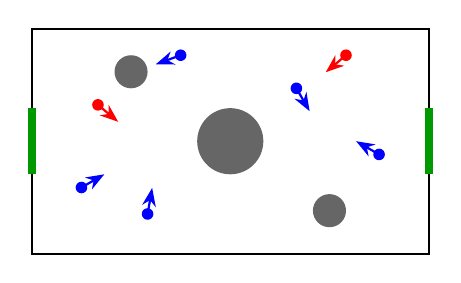
\begin{tikzpicture}[scale=4.2, >=Stealth]
        \draw[thick] (0,0) rectangle (1.2,0.68);
        \draw[green!60!black, line width=3pt] (0,0.24) -- (0,0.44);
        \draw[green!60!black, line width=3pt] (1.2,0.24) -- (1.2,0.44);
        \fill[black!60] (0.6,0.34) circle (0.10);
        \fill[black!60] (0.3,0.55) circle (0.05);
        \fill[black!60] (0.9,0.13) circle (0.05);
        \foreach \x/\y/\a in {0.15/0.2/30, 0.45/0.6/200, 0.8/0.5/-60, 1.05/0.3/150, 0.35/0.12/80}
          {\fill[blue] (\x,\y) circle (0.0175); \draw[->,blue,thick] (\x,\y) -- ++(\a:0.08);}
        \foreach \x/\y/\a in {0.2/0.45/-40, 0.95/0.6/220}
          {\fill[red] (\x,\y) circle (0.0175); \draw[->,red,thick] (\x,\y) -- ++(\a:0.08);}
      \end{tikzpicture}
    \end{column}
  \end{columns}
\end{frame}

\begin{frame}{Modelo: partículas con masa}
  % Choques tal como los calcula el motor (Collisions.java): impulso J entre partículas,
  % reflexión v - 2 (v·ê_n) ê_n contra obstáculo (bounceObstacle) e inversión en paredes.
  \setlength{\jot}{1pt}
  \begin{itemize}\setlength{\itemsep}{0.3em}
    \item Movimiento de partículas:
      \[
        \vect{r}_i(t) = \vect{r}_i(t_0) + \vect{v}_i\,(t - t_0)
      \]
    \item Choques elásticos:
  \end{itemize}
  \small
  \setlength{\abovedisplayskip}{3pt}\setlength{\belowdisplayskip}{3pt}
  \setlength{\abovedisplayshortskip}{3pt}\setlength{\belowdisplayshortskip}{3pt}
  \begin{columns}[T,onlytextwidth]
    \begin{column}{0.42\textwidth}
      \textbf{Partícula $i$ -- partícula $j$}
      \begin{gather*}
        J = \frac{2\,m_i m_j\,(\Delta\vect{v}\cdot\Delta\vect{r})}{\sigma\,(m_i + m_j)}\\
        \vect{v}_i' = \vect{v}_i + \frac{J}{m_i}\,\frac{\Delta\vect{r}}{\sigma}, \qquad
        \vect{v}_j' = \vect{v}_j - \frac{J}{m_j}\,\frac{\Delta\vect{r}}{\sigma}
      \end{gather*}
    \end{column}
    \begin{column}{0.34\textwidth}
      \textbf{Partícula -- obstáculo fijo}
      \[
        \vect{v}' = \vect{v} - 2\,(\vect{v}\cdot\hat{\vect{e}}_n)\,\hat{\vect{e}}_n
      \]
      {\footnotesize $\hat{\vect{e}}_n$: versor normal al choque, del centro del obstáculo al
      de la partícula.}
    \end{column}
    \begin{column}{0.20\textwidth}
      \textbf{Partícula -- pared}\par\vspace{0.6em}
      Vertical:\\ $(v_x, v_y) \to (-v_x, v_y)$\par\vspace{0.5em}
      Horizontal:\\ $(v_x, v_y) \to (v_x, -v_y)$
    \end{column}
  \end{columns}
\end{frame}

% ==========================================================================
\section{Implementación}
% Solo el motor. Sin post-proceso ni I/O.
% ==========================================================================

\begin{frame}{Motor: cola de eventos}
  \begin{columns}[c,onlytextwidth]
  \begin{column}{0.8\textwidth}
  \centering
  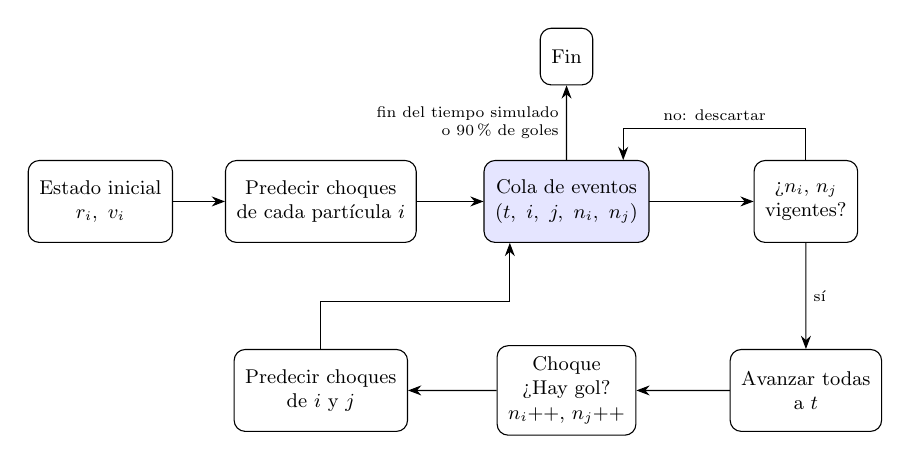
\begin{tikzpicture}[>=Stealth, font=\small, scale=0.8, every node/.append style={scale=0.8},
      caja/.style={draw, rounded corners, align=center, inner sep=5pt, minimum height=1.3cm},
      clave/.style={caja, fill=blue!10}]
    \node[caja]  (ini)  at (0, 0)      {Estado inicial\\ $\vect{r}_i,\ \vect{v}_i$};
    \node[caja]  (pred0) at (3.5, 0)   {Predecir choques\\ de cada partícula $i$};
    \node[clave] (pq)   at (7.4, 0)    {Cola de eventos\\ $(t,\ i,\ j,\ n_i,\ n_j)$};
    \node[caja]  (vig)  at (11.2, 0)   {¿$n_i$, $n_j$\\ vigentes?};
    \node[caja]  (adv)  at (11.2, -3)  {Avanzar todas\\ a $t$};
    \node[caja]  (col)  at (7.4, -3)   {Choque\\ ¿Hay gol?\\ $n_i{+}{+}$, $n_j{+}{+}$};
    \node[caja]  (pred) at (3.5, -3)   {Predecir choques\\ de $i$ y $j$};
    \node[caja, minimum height=0.9cm] (fin) at (7.4, 2.3) {Fin};
    \draw[->] (ini) -- (pred0);
    \draw[->] (pred0) -- (pq);
    \draw[->] (pq) -- (vig);
    \draw[->] (vig) -- node[right, font=\scriptsize] {sí} (adv);
    \draw[->] (vig.north) -- ++(0,0.5) -| node[pos=0.25, above, font=\scriptsize] {no: descartar}
      ($(pq.north)+(0.9,0)$);
    \draw[->] (pq.north) -- node[left, font=\scriptsize, align=right] {fin del tiempo simulado\\ o 90\,\% de goles} (fin);
    \draw[->] (adv) -- (col);
    \draw[->] (col) -- (pred);
    \draw[->] (pred.north) -- ++(0,0.75) -| ($(pq.south)+(-0.9,0)$);
  \end{tikzpicture}
  \end{column}
  \begin{column}{0.2\textwidth}
    \footnotesize\leftskip=0.5cm
    $i$, $j$: partículas\\[0.6em]
    $n_i$: número de choques de la partícula $i$\\[0.6em]
    $t$: instante del evento
  \end{column}
  \end{columns}
\end{frame}

% ==========================================================================
\section{Simulaciones}
% ==========================================================================

\begin{frame}{Sistema}
  \begin{columns}[c]
    \begin{column}{0.54\textwidth}
      \centering
      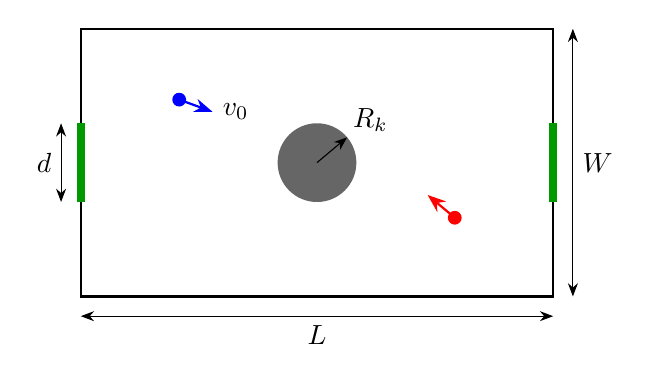
\begin{tikzpicture}[scale=5.0, >=Stealth]
        \draw[thick] (0,0) rectangle (1.2,0.68);
        \draw[green!60!black, line width=3pt] (0,0.24) -- (0,0.44);
        \draw[green!60!black, line width=3pt] (1.2,0.24) -- (1.2,0.44);
        \draw[<->] (0,-0.05) -- (1.2,-0.05) node[midway, below] {$L$};
        \draw[<->] (1.25,0) -- (1.25,0.68) node[midway, right] {$W$};
        \draw[<->] (-0.05,0.24) -- (-0.05,0.44) node[midway, left] {$d$};
        \fill[black!60] (0.6,0.34) circle (0.10);
        \draw[->] (0.6,0.34) -- ++(40:0.10) node[pos=1, anchor=south west, inner sep=2pt] {$R_k$};
        \fill[blue] (0.25,0.5) circle (0.0175);
        \draw[->,blue,thick] (0.25,0.5) -- ++(-20:0.09) node[right, black] {$v_0$};
        \fill[red] (0.95,0.2) circle (0.0175);
        \draw[->,red,thick] (0.95,0.2) -- ++(140:0.09);
      \end{tikzpicture}
    \end{column}
    \begin{column}{0.44\textwidth}
      \textbf{Fijos}
      \begin{itemize}\setlength{\itemsep}{2pt}
        \item $L = 1.20\uni{m}$, $W = 0.68\uni{m}$, $d = 0.20\uni{m}$
        \item $r = 0.0175\uni{m}$, $m = 0.025\uni{kg}$, $v_0 = 1\uni{m/s}$
        \item Posiciones iniciales al azar
      \end{itemize}
      \vspace{0.5em}
      \textbf{Variables}
      \begin{itemize}\setlength{\itemsep}{2pt}
        \item Mesa vacía: 7 valores de $N$ entre 25 y 400
        \item Con obstáculos: $N = 100$, obstáculos $(x_k, y_k, R_k)$
      \end{itemize}
    \end{column}
  \end{columns}
\end{frame}

\begin{frame}{Observables}
  \begin{columns}[c]
    \begin{column}{0.58\textwidth}
      \begin{itemize}\setlength{\itemsep}{0.8em}
        \item $N_g(t)$: cantidad de goles acumulados.
        \item $F_g(t) = N_g(t)/N$.
        \item \textbf{Tiempo al 90\,\%}: $t_{90} = \min\{t : F_g(t) \ge 0.9\}$.
        \item \textbf{Observable}: $\langle t_{90} \rangle$, promedio de $t_{90}$ sobre 20
          realizaciones.
        \item \textbf{Tiempo de ejecución}: promedio sobre 20 realizaciones de $30\uni{s}$
          simulados.
      \end{itemize}
    \end{column}
    \begin{column}{0.40\textwidth}
      \centering
      % Gol: la particula azul llega al arco (verde) y sale roja.
      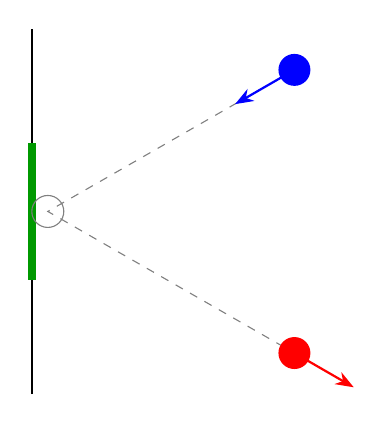
\begin{tikzpicture}[scale=2.9, >=Stealth]
        \draw[thick] (0,0) -- (0,1.6);
        \draw[green!60!black, line width=3pt] (0,0.5) -- (0,1.1);
        \draw[dashed, gray] (1.15,1.42) -- (0.07,0.8) -- (1.15,0.18);
        \draw[gray] (0.07,0.8) circle (0.07);
        \fill[blue] (1.15,1.42) circle (0.07);
        \draw[->,blue,thick] (1.15,1.42) -- ++(210:0.3);
        \fill[red] (1.15,0.18) circle (0.07);
        \draw[->,red,thick] (1.15,0.18) -- ++(-30:0.3);
      \end{tikzpicture}
    \end{column}
  \end{columns}
\end{frame}

\begin{frame}{Observables: difusión}
  \begin{columns}[c]
    \begin{column}{0.52\textwidth}
      \begin{itemize}\setlength{\itemsep}{0.8em}
        \item \textbf{Desplazamiento cuadrático medio}:
          \[
            \mathrm{DCM}(t) = \frac{1}{N}\sum_{i=1}^{N} |\vect{r}_i(t) - \vect{r}_i(0)|^2
          \]
        \item \textbf{Difusión}: $\mathrm{DCM} = 4\,D\,t$. Se marca a ojo el tramo
          $[0, t_{\mathrm{fin}}]$ del ajuste lineal y $D$ minimiza
          $\sum_j [\mathrm{DCM}(t_j) - 4\,D\,t_j]^2$. Promedio sobre 20 realizaciones.
      \end{itemize}
    \end{column}
    \begin{column}{0.46\textwidth}
      \centering
      % Trayectoria de una particula entre choques y su desplazamiento neto.
      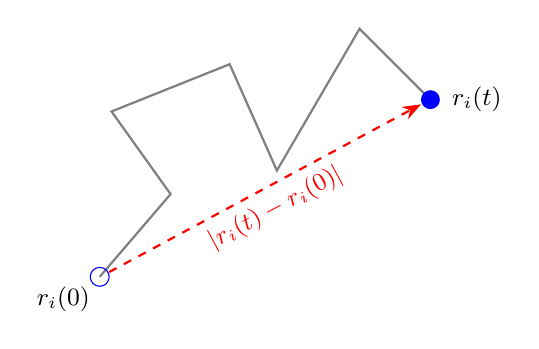
\begin{tikzpicture}[scale=3.0, >=Stealth]
        \draw[gray, thick] (0,0) -- (0.3,0.35) -- (0.05,0.7) -- (0.55,0.9) -- (0.75,0.45)
          -- (1.1,1.05) -- (1.4,0.75);
        \draw[blue] (0,0) circle (0.04);
        \node[below left, font=\small] at (0,0) {$\vect{r}_i(0)$};
        \fill[blue] (1.4,0.75) circle (0.04);
        \node[right, font=\small] at (1.45,0.75) {$\vect{r}_i(t)$};
        \draw[->, red, thick, dashed] (0.04,0.02) -- node[sloped, below, font=\small]
          {$|\vect{r}_i(t) - \vect{r}_i(0)|$} (1.36,0.73);
      \end{tikzpicture}
    \end{column}
  \end{columns}
\end{frame}

\begin{frame}{Configuraciones: disco central}
  \figuraparam[0.78\textwidth]{pres_configs_single_R.png}{%
    Variable: radio $R$
  }
\end{frame}

\begin{frame}{Configuraciones: bloque central}
  \figuraparam[0.78\textwidth]{pres_configs_multi_barrier.png}{%
    Discos de $R = 0.02\uni{m}$\\[0.3em]
    Variable: cantidad de columnas $k$
  }
\end{frame}

\begin{frame}{Configuraciones: bloque con filas}
  \figuraparam[0.78\textwidth]{pres_configs_multi_barrier_rows.png}{%
    Discos de $R = 0.02\uni{m}$\\[0.3em]
    Variables: columnas $k$,\\ filas por lado $n$
  }
\end{frame}

% ==========================================================================
\section{Resultados}
% 1.1, despues el 1.2 por familia: animacion -> F_g(t) -> <t_90> vs variable (esquemas de cada
% familia en Simulaciones); cierra con la mejor de cada familia y la elegida. Despues el 1.3.
% ==========================================================================

\begin{frame}{Tiempo de ejecución vs $N$}
  \figura{time_vs_n.png}
\end{frame}

% --- Disco central ---------------------------------------------------------

\begin{frame}{Disco central: animación}
  \begin{columns}[c,onlytextwidth]
    \begin{column}{0.5\textwidth}
      \animbox{snapshot_empty.png}{Mesa vacía}{\yt{YCpG6rdYMtU}}
    \end{column}
    \begin{column}{0.5\textwidth}
      \animbox{snapshot_disco.png}{$R = 0.33\uni{m}$}{\yt{OzH415fexjk}}
    \end{column}
  \end{columns}
\end{frame}

\begin{frame}{Disco central: fracción de goles vs tiempo}
  \figura{fg_empty_disco.png}
\end{frame}

\begin{frame}{Disco central: $\langle t_{90} \rangle$ vs radio}
  \figura{t90_single_R.png}
\end{frame}

% --- Bloque central --------------------------------------------------------

\begin{frame}{Bloque central: animación}
  \animsola{snapshot_mb_k16.png}{$k = 16$}{\yt{PENDIENTE}}
\end{frame}

\begin{frame}{Bloque central: fracción de goles vs tiempo}
  \figura{fg_multi_barrier.png}
\end{frame}

\begin{frame}{Bloque central: $\langle t_{90} \rangle$ vs cantidad de columnas}
  \figura{t90_multi_barrier.png}
\end{frame}

% --- Bloque con filas ------------------------------------------------------

\begin{frame}{Bloque con filas: animación}
  \animsola{snapshot_elegida.png}{$k = 17$, $n = 1$}{\yt{wTY2R0gUhOo}}
\end{frame}

\begin{frame}{Bloque con filas: fracción de goles vs tiempo}
  \figuraparam[0.78\textwidth]{fg_rows.png}{%
    $k = 17$
  }
\end{frame}

\begin{frame}{Bloque con filas: $\langle t_{90} \rangle$ vs filas}
  \figura{t90_multi_barrier_rows_k.png}
\end{frame}

% --- Cierre del 1.2 --------------------------------------------------------

\begin{frame}{Mejor configuración de cada familia}
  \figuraparam[0.72\textwidth]{t90_best.png}{%
    Disco central:\\ $R = 0.33\uni{m}$\\[0.5em]
    Bloque central:\\ $k = 18$\\[0.5em]
    Bloque con filas:\\ $k = 17$, $n = 1$
  }
\end{frame}

\begin{frame}{Configuración elegida}
  \figuraparam[0.72\textwidth]{pres_config_elegida.png}{%
    $k = 17$, $n = 1$\\[0.3em]
    $K = 245$ discos de $R = 0.02\uni{m}$\\[0.6em]
    $\langle t_{90} \rangle = 13.6 \pm 1.8\uni{s}$
  }
\end{frame}

\begin{frame}{Difusión: DCM vs tiempo}
  \centering
  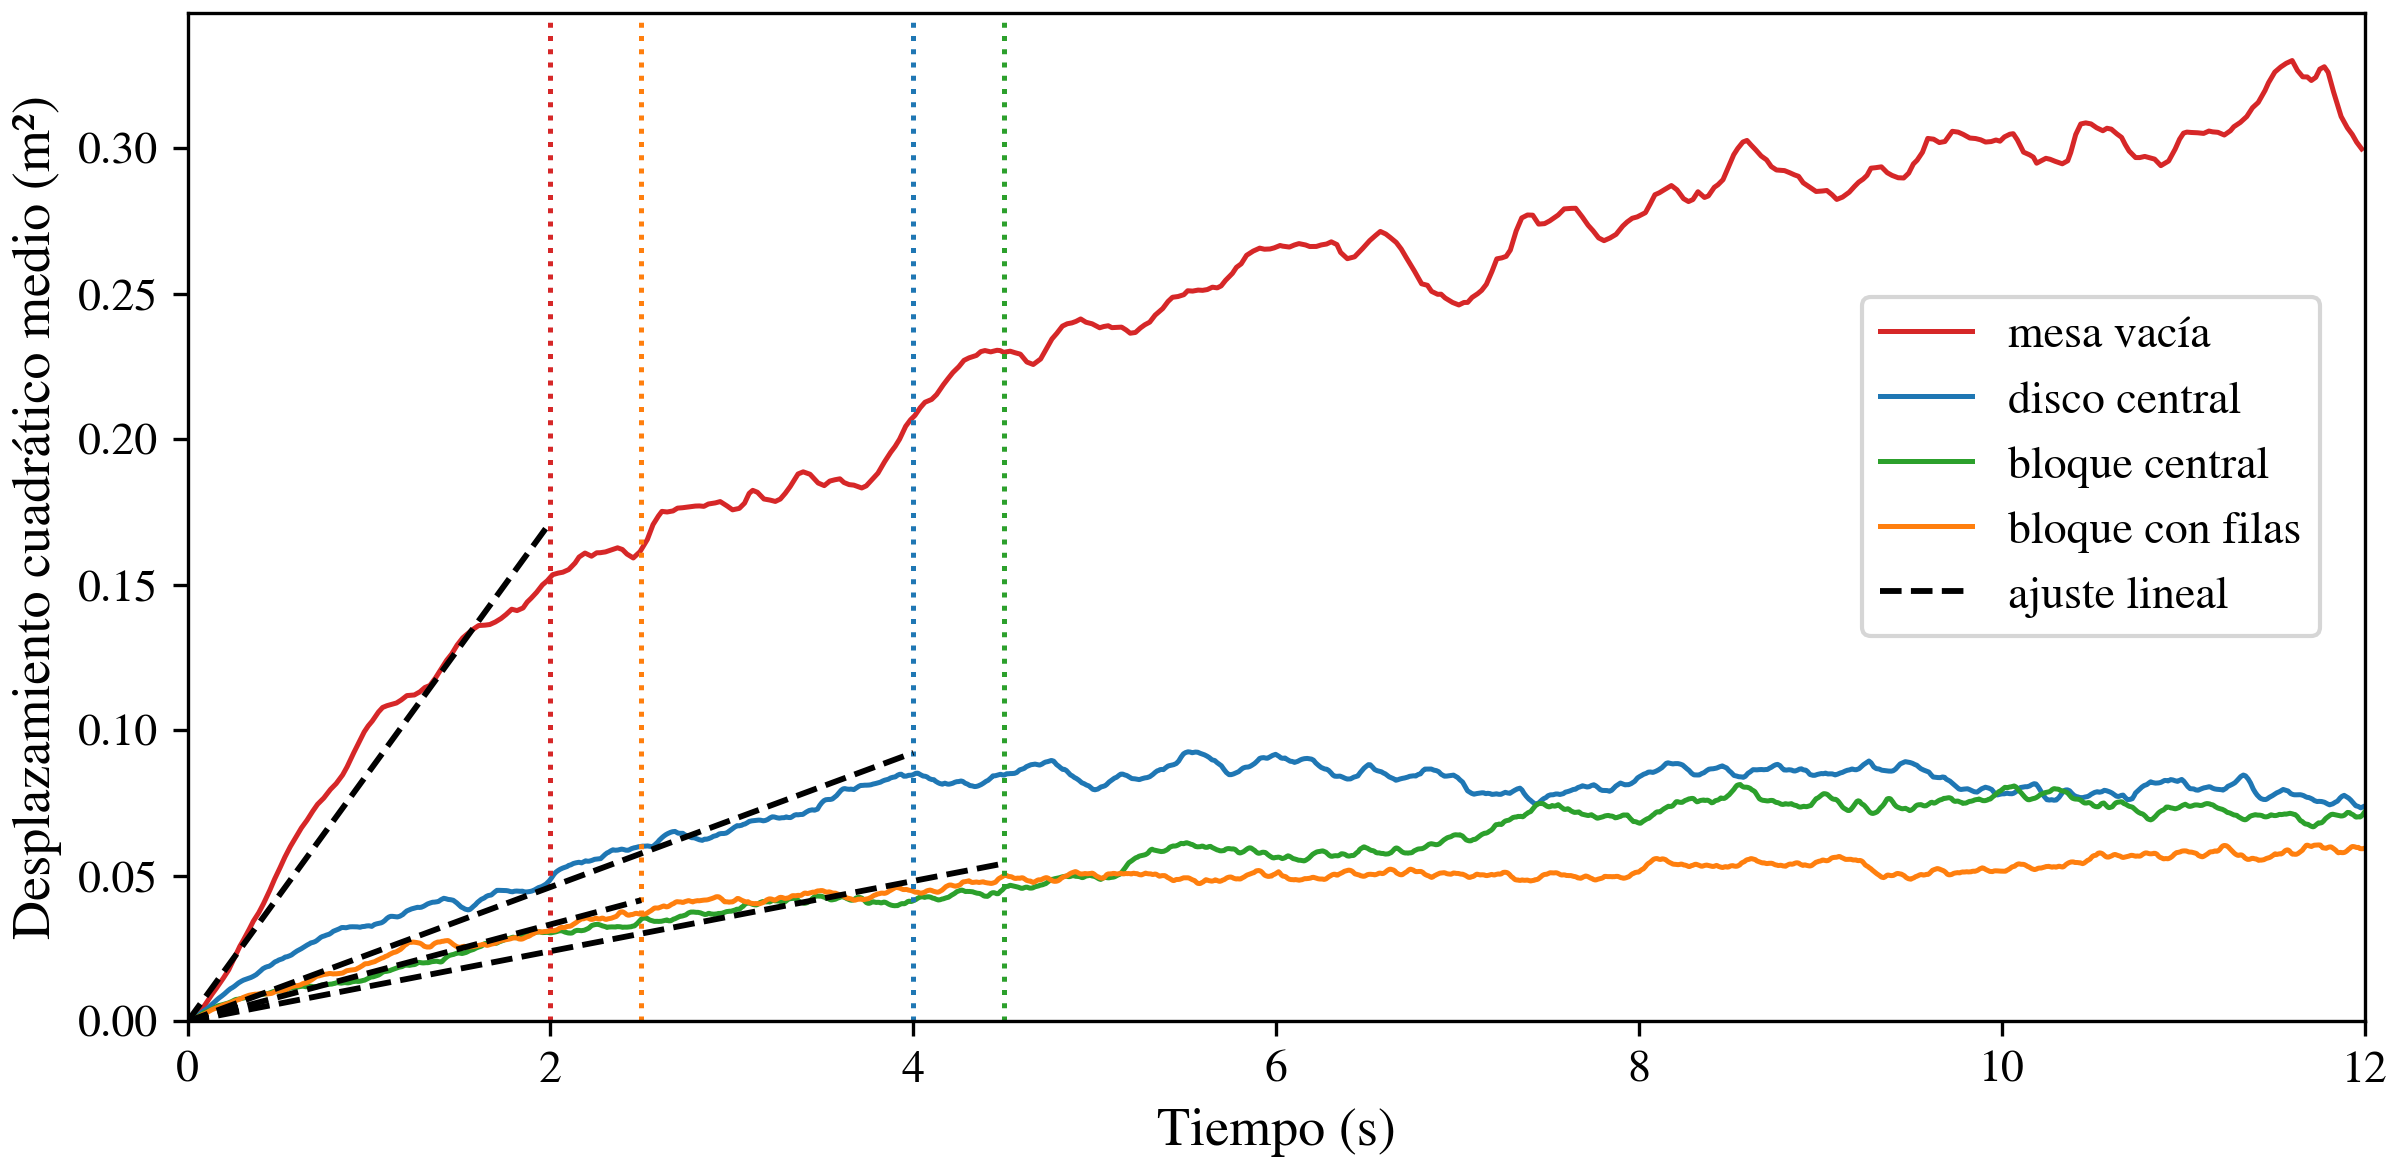
\includegraphics[width=\linewidth,height=0.9\textheight,keepaspectratio]{dcm_vs_t.png}
\end{frame}

\begin{frame}{$\langle D \rangle$ vs $\langle t_{90} \rangle$}
  \figura{D_vs_t90.png}
\end{frame}

\begin{frame}{Bloque central: $\langle D \rangle$ vs $\langle t_{90} \rangle$}
  \figura{D_vs_t90_multi_barrier.png}
\end{frame}

% ==========================================================================
\section{Conclusiones}
% Solo lo que está en las figuras de Resultados. Cuantificar.
% ==========================================================================

\begin{frame}{Conclusiones}
  \begin{itemize}
    \item Distintas configuraciones de obstáculos reducen $\langle t_{90} \rangle$ respecto de la
      mesa vacía.
    \item Comprimir el espacio mejora $\langle t_{90} \rangle$; demasiada compresión lo vuelve a
      aumentar.
    \item A mayor espacio, mayor movimiento de las partículas: mayor DCM y mayor $D$.
  \end{itemize}
\end{frame}

\begin{frame}[plain]
  \centering
  \vfill
  {\Huge Muchas gracias}
  \vfill
\end{frame}

\end{document}
